%%%%%%%%%%%%%%%%%%%%%%%%%%%%%%%%%%%%%%%%%%%%%%%%%%%%%%%%%
\chapter[Arborescence du projet]{Arborescence du projet}
\label{chap:chap7}

L'arborescence du projet est la suivante:

\begin{description}
 \item[arduino\_wrapper: ] les sources de nos portages.
 \item[docs: ] contient l’ensemble des documents utiles des projets.
 \item[elua: ] contient les sources eLua.
 \item[env: ] le dossier contient les outils indispensables pour la compilation (sourcerytoolchain g++) et le flash de la carte.
 \item[examples: ] contient les exemples documentés prêts à l’emploi.
\end{description}
 
\begin{figure}[h]
\begin{center}
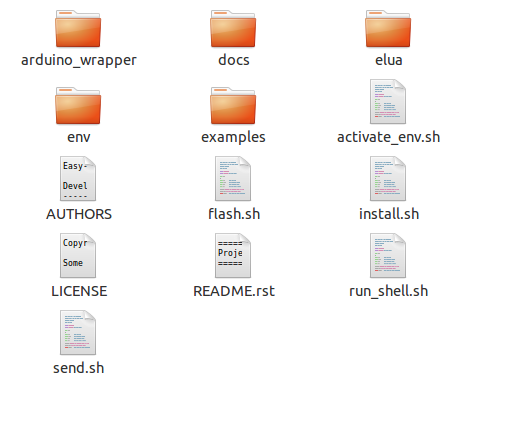
\includegraphics[scale=0.6]{figure/arborescence.png}
\caption{Arborescence du projet}
\end{center}
\end{figure}

L’une des fonctionnalités intéressantes du projet, est l’installation automatique de l’environnement de développement. 
En effet, le script ``install.sh'' permet d’automatiser cette tâche rendant plus simple le premier contact avec Easy-eLua.

Nous avons également développé d’autres scripts pour automatiser d’autres tâches, comme le flash de la carte avec un programme 
Easy-eLua ou encore l’envoi de celui-ci sur une carte possédant déjà un environnement eLua.